% Q19：正三棱柱及题问直线 CA_1 的示意透视图，按源图虚实线关系绘制，不按比例。
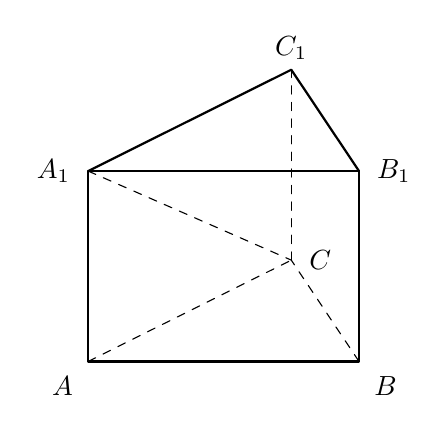
\begin{tikzpicture}[x=0.86cm,y=0.78cm,line cap=round,line join=round]
  \coordinate (A) at (0,0);
  \coordinate (B) at (4,0);
  \coordinate (C) at (3,1.65);
  \coordinate (A1) at (0,3.1);
  \coordinate (B1) at (4,3.1);
  \coordinate (C1) at (3,4.75);

  % Hidden base edges, rear prism edge, and the queried line CA_1.
  \draw[dashed] (A)--(C);
  \draw[dashed] (B)--(C);
  \draw[dashed] (C)--(C1);
  \draw[dashed] (A1)--(C);

  % Visible front rectangle and upper triangular face.
  \draw[thick] (A)--(B)--(B1)--(A1)--cycle;
  \draw[thick] (A1)--(C1)--(B1);

  \node[below left=2pt] at (A) {$A$};
  \node[below right=2pt] at (B) {$B$};
  \node[right=3pt] at (C) {$C$};
  \node[left=3pt] at (A1) {$A_1$};
  \node[right=3pt] at (B1) {$B_1$};
  \node[above] at (C1) {$C_1$};
\end{tikzpicture}
